\section{設計}
\pagenumbering{arabic}

プレイヤーのPCから最も近い利用可能な遊休コンピュータを探し、クラウドゲームサーバをホストさせるシステム

\subsection{提案システムの概要}
提案システムの概要を図\ref{fig:arch}に示す。
プレイヤーPC上のVCクライアントエージェントがクラウド上のVCコントローラにゲームプレイをリクエスト。VCコントローラが遊休コンピュータにVCホストエージェントにクラウドゲームのホスティングをリクエスト。遊休コンピュータでクラウドゲームサーバとゲームが起動し、プレイヤーPC上のクラウドゲームクライアントと通信してゲームをする。

\subsection{VCコントローラ}
クラウド上に存在するVCコントローラはゲームをプレイしたいプレイヤーのPCと利用可能な遊休コンピュータをマッチングする役割を果たす。プレイヤーPCからのゲームプレイのリクエストを受け取ると、利用可能な遊休コンピュータ群の中からプレイヤーPCからのネットワーク遅延が小さいものを見つける。そしてその遊休コンピュータに対してクラウドゲームのホスティングをリクエストする。また、このマッチングの成立後、VCコントローラはVCクライアントエージェントとVCホストエージェントにクラウドゲームサーバ/クライアントが通信するためのリンクを張るのに必要な情報を配布する。

\subsection{VCクライアントエージェント}
VCクライアントエージェントはボランティアクラウドゲーミングコントローラ上のVCコントローラへゲームプレイのリクエストを送信する。このときプレイしたいゲームやサーバとリンクを張るために必要なネットワーク情報などを付帯して送信する。

\subsection{VCホストエージェント}
VCコントローラに割り当てられた遊休コンピュータ上のVCホストエージェントはクラウドゲームのホスティングのリクエストを受け取る。その後クラウドゲームサーバとゲームを起動し、接続に必要な情報と共にVCクライアントエージェントに起動完了のメッセージを送信する。

\subsection{クラウドゲームサーバ/クライアント}
クラウドゲームサーバはゲーム画面をキャプチャして、ビデオストリームとしてクラウドゲームクライアントに送信する。一方で、クラウドゲームクライアントは受け取ったゲーム画面の描画を行う。また、クラウドゲームクライアントはプレイヤーの入力操作をキャプチャしてクラウドゲームサーバ上のゲームの入力となるように送信を行う。

\begin{figure*}[t]
    \centering
    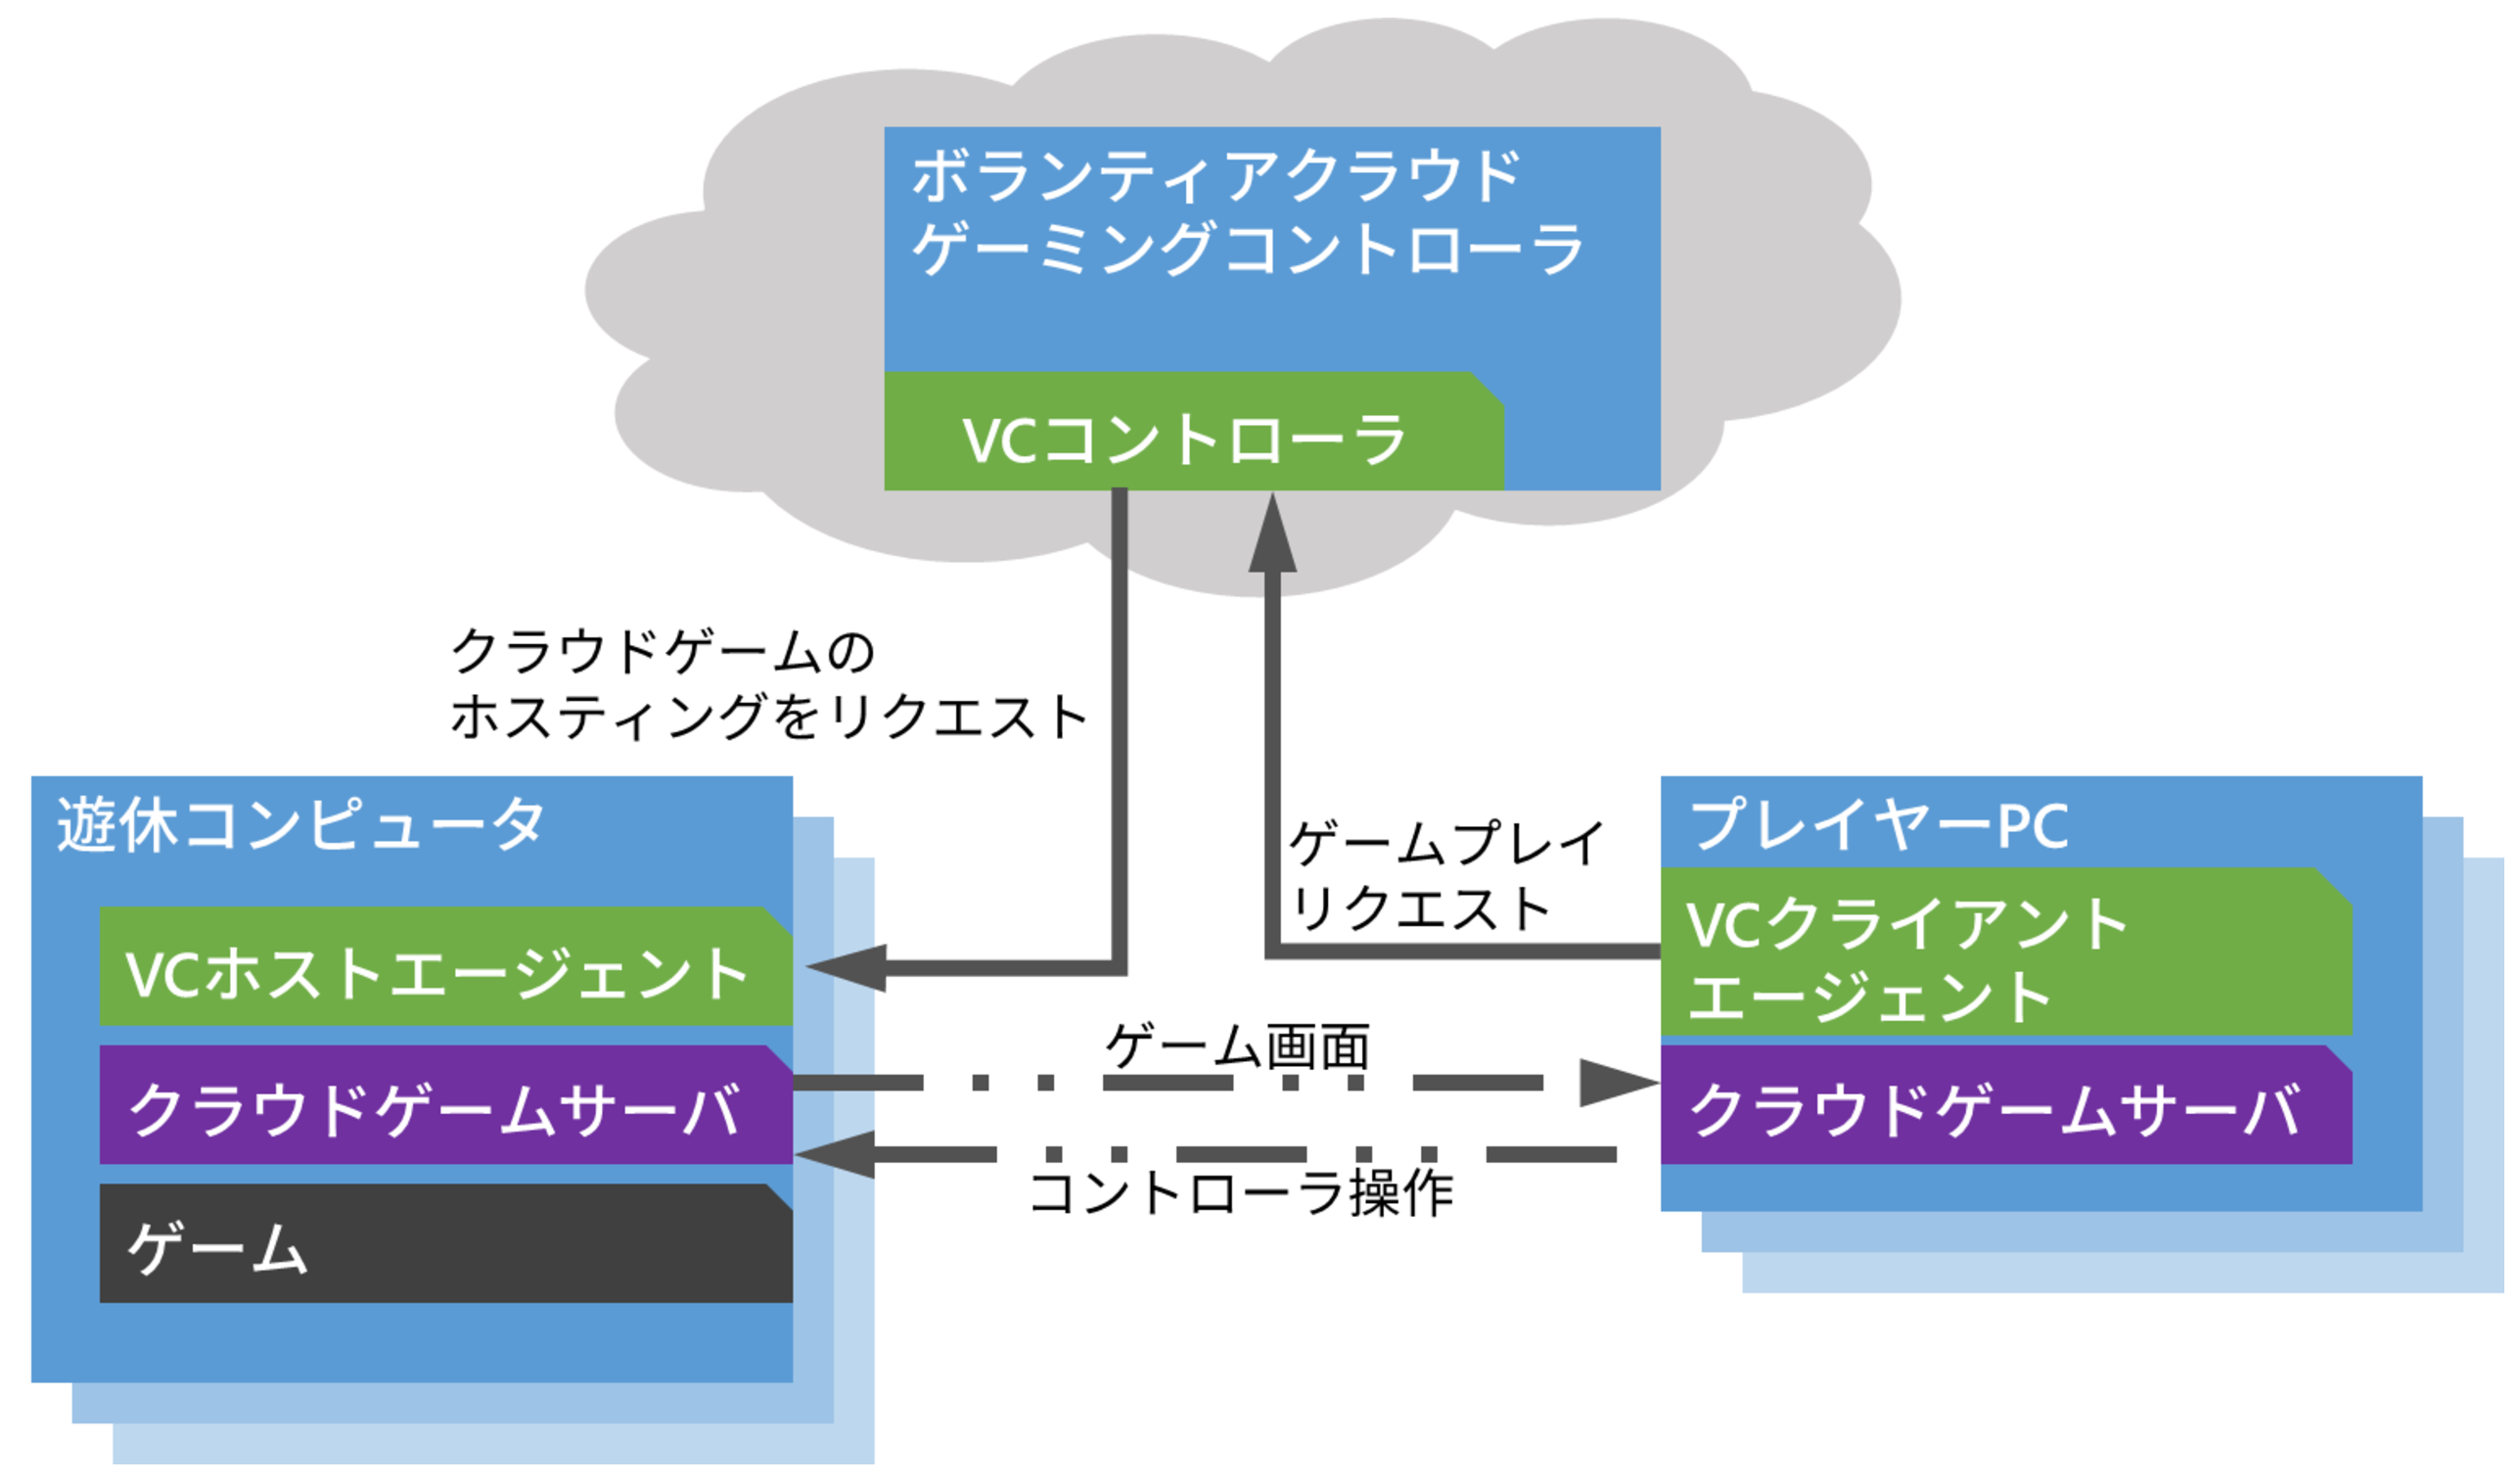
\includegraphics[width=0.8\textwidth,keepaspectratio,clip]{img/architecture.eps}
    \caption{アーキテクチャ}
    \label{fig:arch}
\end{figure*}
